%% Ggf. folgende Zeile auskommentieren, falls der Sperrvermerk gewünscht ist.
%\chapter*{Sperrvermerk} %*-Variante sorgt dafür, das der Sperrvermerk nicht im Inhaltsverzeichnis auftaucht
%Der Inhalt dieser Arbeit darf weder als Ganzes noch in Auszügen Personen außerhalb des Prüfungsprozesses und des Evaluationsverfahrens zugänglich gemacht werden, sofern keine anders lautende Genehmigung vom Dualen Partner vorliegt.
%
%Musterstadt, den \today \\[4ex]
%
%\rule[-0.2cm]{5cm}{0.5pt} \\
%
%\textsc{\autor} \\[10ex]

\chapter*{Erklärung} %*-Variante sorgt dafür, dass die Erklärung nicht im Inhaltsverzeichnis auftaucht

Wir versichern hiermit, dass wir unsere \arbeit\ mit dem Thema:

\begin{quote}
	\textit{\titel} % -\textit{ \untertitel }
\end{quote}

selbstständig verfasst und keine anderen als die angegebenen Quellen und Hilfsmittel benutzt haben. \\[0ex]

Rüsselsheim, den \today \\[0ex]

%\rule[-0.2cm]{5cm}{0.5pt} \\




\includegraphics[width=4cm]{images/AngusBach.jpg} \hspace{1.5cm} \textsc{Angus Bach}\\[0em]

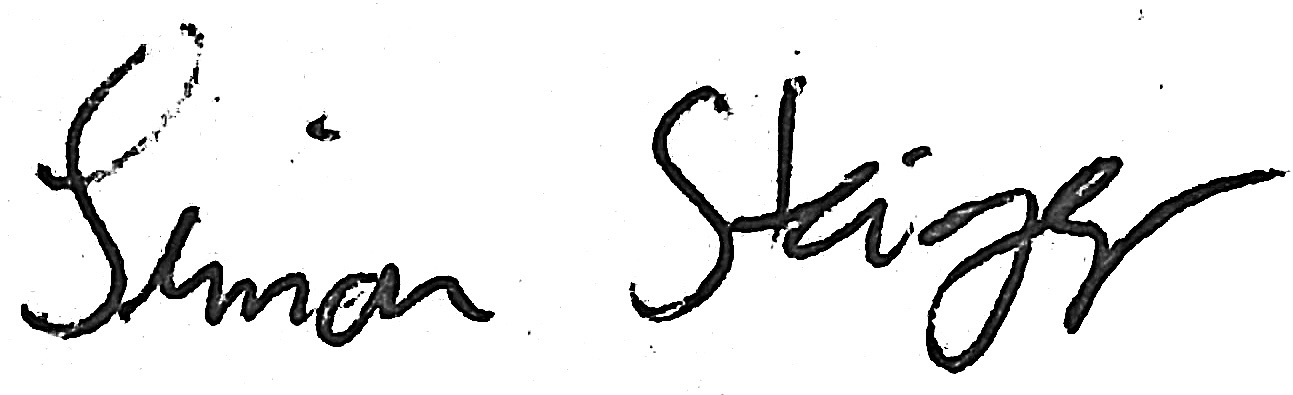
\includegraphics[width=4cm]{images/SimonSteiger.jpg} \hspace{1.5cm} \textsc{Simon Steiger}\\[0em]


\includegraphics[width=4.8cm]{images/HaiNamNguyen.jpg} \hspace{0.7cm} \textsc{Hai Nam Nguyen}\\[0em]

%\autor \\[10ex]

\rmfamily

\thispagestyle{empty}

